\def\ChineseVersion{1}
\documentclass[10pt,twocolumn]{article}
\usepackage{paper-style}
\author{Francis Du}
\hypersetup{pdfauthor={Francis Du},pdftitle={WCode：面向有状态软件智能体的修订绑定证据},pdfsubject={软件工程运行时与证据适用性}}
\begin{document}
\paperheading{WCode：面向有状态软件智能体的\\修订绑定证据}{2026 年 11 月 6 日}{%
软件智能体通过一系列仓库读取、编辑、检查和验收决策开展工作。某一步产生的证据可能在代码或设计变更后失去适用性，而一个生产者给出的成功检查结果也可能掩盖另一个生产者的冲突结果。本文介绍 Rust 运行时 \wcode{}，它将这些边界显式化。其核心抽象是修订绑定证据：观察记录保留对象、生产者、权威性、覆盖范围以及代码与设计修订，由策略决定其能否支持当前操作。该运行时结合了有界源码交付、基于乐观并发控制的文件修改、验证复用以及保留生产者区分的协调核对。本文给出由此形成的准入契约，并使用冻结的可执行文件考察其实现。无模型诊断覆盖四种语言的 60 个合成场景、三档响应预算、两个执行框架缓存阶段和七次重复，共产生 2,520 次实测查询。选定的 22 项契约反例在同一可执行文件上成功重放，十一项运行控制检查也全部通过。在每种诊断条件下，全部 686 个必需源码实例和全部 406 项符合条件的编辑输入均得到交付。然而，序列化决策记录的对外暴露率从 0\% 到 70\% 不等；从就绪判定谓词中移除可写性条件后，每种条件下的 413 次可回答观察中均出现七个假阳性。这些结果说明，成功检索与可执行操作的就绪状态需要分别测量。结果支持本次测试所覆盖的运行时契约；能否推广到真实仓库的问题修复，仍需实证检验。}
\section{引言}
\label{sec:introduction}
面向仓库的软件智能体正日益将代码检索、编辑、命令执行和反馈整合进同一工作流。SWE-bench 衡量完整系统解决真实仓库问题的能力，SWE-agent 和 OpenHands 则展示了语言模型周围的接口与执行环境的重要性 \cite{jimenez2024swebench,yang2024sweagent,wang2025openhands}。这些系统使另一个问题变得至关重要：当智能体依据先前观察到的结果采取行动时，什么将该结果与即将被修改的软件状态联系起来？

设想一个智能体正在修改会话刷新行为。它定位到正确的函数并取得源码，随后另一工作者更新了同一文件。此时，先前修订的测试结果仍可获取；第二个验证器针对更窄的目标报告通过；实现任务也被标记为完成。这些观察并不一定有误。错误发生在它们各自不同的含义被合并为一个信号，进而被理解为当前变更已经就绪之时。定位成功不能证明编辑所依据的源码仍是当前版本；执行过检查不能证明所有需求都已被覆盖；任务完成也不能证明验收通过。

本文从运行时边界研究这一协调问题。我们将\emph{证据}定义为针对工件或操作的带类型观察，其中记录了来源和适用条件。证据不再足以证明某项当前操作合理之后，仍可能作为历史记录发挥作用。因此，关键区别在于保留一项观察与将其纳入当前决策之间。只要智能体、人工编辑者和后台检查共同使用持续演化的软件状态，这一区别就至关重要。

本文提出 \wcode{}，这是一个已实现的 Rust 运行时，通过模型上下文协议（Model Context Protocol）提供接口。它维护软件意图声明、代码观察、验证记录和工作项状态。其组织原则是：操作所使用的证据必须具有明确的适用条件。读取操作返回原始源码与文件身份；修改操作将当前文件与已观察的身份进行核对；验证操作记录检查执行时绑定的修订与权威性；协调核对则保留生产者之间与当前操作相关的分歧。同一原则也决定接口应将哪些内容报告为缺失或不确定。

本文的研究问题是：\emph{共享的软件智能体运行时，如何在有界观察、并发修改与验证之间保持证据的适用性？} 本文通过以下三项贡献考察这一问题：
\begin{enumerate}
\item 给出明确的准入契约，将证据与代码和设计修订、目标范围、权威性及策略关联起来。该契约区分支持当前决策的证据、历史观察以及尚未解决的生产者冲突。
\item 实现一个运行时，将这些区别贯穿于上下文打包、受保护的单文件编辑、验证执行与复用以及协调核对。贯穿示例说明，为何必须在每个边界保留这些字段。
\item 提供可审计的诊断评估，分别测量源码交付、编辑输入就绪状态、运行控制和描述性开销。保留的可执行文件与源码归档标识主试验运行；通过移除谓词条件的分析，揭示被饱和检索分数掩盖的就绪判定错误。
\end{enumerate}

本文的贡献是围绕共享操作契约对已有机制进行组合。哈希、来源记录、架构一致性和访问控制均已有大量研究；第~\ref{sec:related} 节将本运行时置于这些研究脉络中。相应地，本文评估的范围也是明确限定的：评估不调用语言模型，只确认开发者编写的场景中的行为，不证明补丁成功率有所提高。这一范围使我们能够直接考察工具边界上的失败，而不将其归因于模型推理；对下游有效性的评估则留待独立实验。

\section{证据准入契约}
\label{sec:contract}
\subsection{状态与观察}
设工作区状态为
\begin{equation}
 S=(D,C,P,G,E,W),
\end{equation}
其中，$D$ 为设计声明，$C$ 为代码，$P$ 为适用策略，$G$ 为已观察的软件图，$E$ 为证据历史，$W$ 为工作项状态。其修订表示为 $\rho(S)=(\rho_C,\rho_D)$，其中设计分量可选。策略单独绑定，不是第三个修订字段。将设计纳入修订很有必要，因为即使代码字节未变，验收标准的变化也可能使先前结果不再适用。

为便于说明，将证据记录表示为
\begin{equation}
 e=(u,k,p,\rho,\sigma,a,o,\pi,\tau),
\end{equation}
其中，$u$ 为对象，$k$ 为证据类型，$p$ 为生产者，$\rho$ 为采集时的修订，$\sigma$ 为覆盖目标，$a$ 为权威性，$o$ 为结果，$\pi$ 为相关策略绑定，$\tau$ 为顺序标记或执行回执。该元组概括了分散在实现各处的检查，并不意味着所有子系统都采用同一种记录模式。

来源与权威性的作用不同。生产者标识记录某项观察由谁提供；权威性决定该入口有权确立哪些主张。自报的生产者名称或置信分数不能将外部证据转变为原生验证结果。同样，自动策略授权与明确的人工批准是不同的证据类型。如果把其中任何一组区别都替换成泛化的“成功”，就会改变决策的含义。

\subsection{适用性与生产者冲突}
对于请求 $q$，定义适用证据子集
\begin{align}
 E_q(S)&=\{e\in E:\App(e,S,q)\},\\
 \App(e,S,q)&=\operatorname{Complete}(e.\rho) \nonumber\\
 &\quad\land(e.\rho=\rho(S)) \nonumber\\
 &\quad\land\operatorname{Relevant}(e.\sigma,q) \nonumber\\
 &\quad\land\operatorname{Authorized}(e.a,P,q) \nonumber\\
 &\quad\land\operatorname{Compatible}(e.\pi,P,q).
 \label{eq:applicable}
\end{align}
各谓词的具体含义取决于操作类型。相关性用于纳入涉及请求目标的观察；当某条记录为某项具体要求提供支持时，再检查其确切覆盖范围。兼容性关注与该证据类型相关的策略条件。不完整的修订指纹不能确立与确切修订绑定的原生证据。为便于检查而保留这类记录，并不会使其具备适用性。

仅有适用性仍不足以解决记录之间的冲突。我们依据保留对象、证据类型、生产者和适用范围的键，对各组记录进行归约。只有满足相应的带类型回执规则与覆盖规则时，较新的记录才能取代较旧的记录。令 $L_q$ 表示归约后保留的记录。全局采用“以最新结果为准”的归约并不合适：生产者 $p_2$ 的通过结果不能抹去生产者 $p_1$ 的适用失败记录。

令 $Q$ 为非空的必需检查集合，$A$ 为额外配置的验收门控条件，$\bar S=(D,C,P,G,W)$ 为不含证据历史的状态。一条简化的准入规则为
\begin{align}
 \Accept(S,q) \iff{}& Q\ne\varnothing \nonumber\\
 &\land\ \forall t\in Q:\Pass(t,L_q) \nonumber\\
 &\land\ \nexists e\in L_q:\Fail_q(e) \nonumber\\
 &\land\ \operatorname{GatesSatisfied}(A,\bar S,L_q).
 \label{eq:accept}
\end{align}
这里，$\Pass(t,L_q)$ 要求适用的支持证据，其覆盖范围、类型、权威性与回执均需满足检查 $t$ 的要求；尚未补做的跳过检查不能提供这种支持。$\Fail_q(e)$ 表示请求策略下具有阻断作用的失败，并非泛指所有负面或提示性观察。已配置的门控条件仅通过 $L_q$ 访问证据。实现中区分了检查结果聚合与更大范围的协调核对和验收。式~\eqref{eq:accept} 将它们的逻辑依赖显式化，而不是用单一执行状态标志替代这些区别。

\begin{proposition}[加入无关记录时的保持性]
\label{prop:preservation}
固定 $\bar S$、请求 $q$、必需检查与门控条件，以及归约规则。加入不适用的证据不会改变准入结果。如果生产者 $p_1$ 的一条适用且具有阻断作用的失败记录仍被保留，则加入另一生产者 $p_2$ 的通过记录不能使准入条件变为真。
\end{proposition}
\begin{proof}
不适用记录在归约前即被排除，因此 $L_q$ 不变。检查与门控条件的其他参数均已固定，所以准入结果不变。不同生产者的记录具有不同的归约键，因此新增的通过记录不能取代该阻断失败记录。该失败记录使式~\eqref{eq:accept} 的第三个合取项为假。
\end{proof}

该命题只涉及指定的准入规则，并以输入真实、完整且绑定正确为前提。它不证明测试充分、生产者可信或实现已经得到形式化验证。尤其是，仅凭采集到的修订标签，不能证明某个进程在整个执行期间读取的都是不可变快照。这些假设区分了契约能够保证的性质与证据采集环节必须确立的事实。

\subsection{贯穿示例：一次变更}
表~\ref{tab:trace} 给出会话刷新示例的一条示意轨迹。标识符仅用于说明，不构成额外的实证任务。该轨迹揭示了两个彼此独立的有效性边界：编辑所使用的文件观察，以及验收所使用的修订绑定支持证据。

\begin{table}[t]
\small
\caption{一次变更中的证据状态转移示例。}
\label{tab:trace}
\begin{tabularx}{\columnwidth}{@{}p{0.19\columnwidth}X@{}}
\toprule
事件 & 对后续操作的影响\\
\midrule
读取 $h_0$ & 响应标识函数、原始函数体以及当前文件哈希。\\
其他工作者修改 & 文件状态变为 $h_1$；仍以 $h_0$ 为预期值的编辑必须刷新输入。\\
先前通过 & 当前修订为 $\rho_1$ 时，绑定到 $\rho_0$ 的证据仍作为历史记录保留。\\
$p_1$ 失败 & 当前失败记录在其对象与范围内保持可见。\\
$p_2$ 通过 & 来自另一生产者的通过记录不能取代 $p_1$ 的失败记录。\\
任务结束 & 完成操作更新工作项状态；验收仍需要适用的检查结果和门控条件。\\
\bottomrule
\end{tabularx}
\end{table}

源码摘录、测试通过记录和人工批准之间不存在一种通用排序，使其可以被视为可相互替代的置信度增量。它们支持的是不同谓词。因此，运行时同时公开观察结果和尚待满足的要求，使调用方能够有针对性地重新读取、重新验证或进行审查，而不必从一个未加区分的分数中推断就绪状态。

\section{运行时设计与实现}
\label{sec:implementation}
\wcode{} 通过四项相互连接的职责实现这一契约：观察软件状态、构造有界上下文、判定修改是否准入，以及协调核对验证证据。图~\ref{fig:architecture} 展示了它们之间的关系。运行时不规定调用方使用何种模型或规划策略，而是约束调用方可用操作的含义。

\begin{figure*}[t]
\centering
\begin{tikzpicture}[
  block/.style={draw=inkblue!75,rounded corners=2pt,align=center,inner sep=7pt,font=\small,text width=1.83in,minimum height=.55in},
  store/.style={block,fill=palegray},
  arr/.style={-{Latex[length=2mm]},line width=.6pt,draw=inkblue!90},
  note/.style={font=\footnotesize,fill=white,inner sep=2pt,align=center}]
\node[block] (context) {有界上下文\\身份、源码、文件哈希};
\node[block,right=.44in of context] (edit) {受保护修改\\策略、锁、哈希检查};
\node[block,right=.44in of edit] (verify) {验证\\执行、复用、记录};
\node[store,below=.64in of context] (state) {软件状态\\设计、代码、已观察图};
\node[store,below=.64in of edit] (ledger) {证据历史\\修订、生产者、权威性};
\node[block,below=.64in of verify] (reconcile) {协调核对\\覆盖范围、冲突、门控};
\draw[arr] (context) -- node[note,above]{编辑输入} (edit);
\draw[arr] (edit) -- node[note,above]{新修订} (verify);
\draw[arr] (state) -- node[note,left]{观察} (context);
\draw[arr] (edit.south west) -- node[note,above,sloped]{失效} (state.north east);
\draw[arr] (verify.south west) -- node[note,above,sloped]{回执} (ledger.north east);
\draw[arr] (ledger) -- node[note,above]{适用证据集} (reconcile);
\draw[arr] (state) -- node[note,above]{修订绑定} (ledger);
\draw[arr] (verify) -- node[note,right]{结果} (reconcile);
\end{tikzpicture}
\caption{运行时将证据贯穿于操作边界。源码身份约束修改；修订与来源约束验证复用和协调核对。调用方获得操作结果和尚待满足的要求。历史记录失去适用性后，仍可供检查。}
\label{fig:architecture}
\end{figure*}

\subsection{观察设计与实现}
设计声明表示需求、组件、约束、决策与验收标准。引用将组件连接到文件或符号，并将需求连接到实现与验证目标。这些引用提供可追溯性：解析一个符号能够确立映射关系，而行为本身仍需要适当验证。

软件图将声明与文件、符号、测试、风险和证据关联起来。已观察的关系保留其提供者、精度和修订。因此，来自语法的结构与新鲜的语义提供者结果仍可区分。有界遍历会报告覆盖不完整；存在歧义的符号匹配或多个组件归属会继续作为候选保留。在架构比较中，如果观察不足，未观察到某条边会被记为尚未验证的实际结构，而不会转化为某项依赖确定缺失的结论。

设计准入规则仅适用于已经初始化产品设计的情况。在这一范围内，无效的设计状态或缺失的实现归属可以阻止修改。该规则不要求每个无关工作区都定义产品模型。这一适用范围很重要：如果不满足初始化前提就施加设计门控，原本有用的项目契约就会变成缺乏解释的全局禁令。

\subsection{作为输出契约的有界上下文}
上下文接口汇集任务目标、原始源码、文件元数据、图关系、可用检查和工作项状态。选择阶段优先考虑明确目标与有用的可执行定义；彼此独立的源码项可以并发加载。随后，打包过程压缩可重建的元数据，并裁减较低优先级的内容，以满足明确的响应预算。

对于序列化响应 $y$，计量大小定义为
\begin{equation}
 b(y)=\left\lceil\frac{|\operatorname{JSON}(y)|_{\mathrm{bytes}}}{4}\right\rceil.
 \label{eq:budget}
\end{equation}
请求要求满足 $b(y)\le B$。这一基于字节数的代理量是接口计量规则，不是模型分词器。完整的源码窗口保留原始内容与起止行号；摘要不能替代缺失的原始源码。打包后会刷新就绪状态，因为内部找到的符号可能并未出现在实际交付的响应中。最终序列化结果会再次接受预算检查；无法满足上限时返回错误。

这种以输出为中心的设计形成了一个可测试的不变量：就绪状态必须由调用方实际收到的内容支持。内部检索命中不能证明所交付函数体的覆盖性，当前哈希也不能弥补遗漏的函数体。第~\ref{sec:results} 节分别评估这些谓词。

\subsection{明确范围内的乐观修改}
修改已有文件时，调用方需提供预期的 SHA-256 哈希。准入过程检查写策略、解析路径、获取该文件的锁，再次解析路径，拒绝不受支持的链接条件，并比较当前哈希与预期哈希。运行时验证拟写入内容后，执行原子的单文件替换，并返回修改前后的哈希。算法~\ref{alg:edit} 概括了这一过程。

\begin{algorithm}[t]
\small
\caption{受保护编辑的准入过程（契约抽象）}
\label{alg:edit}
\textbf{输入：} 路径 $f$、已观察哈希 $h$、请求的编辑 $\Delta$\\
\textbf{输出：} 提交前后的哈希，或带类型的拒绝结果
\begin{enumerate}[label=\arabic*.,leftmargin=1.6em]
\item 检查适用的工作区、设计与写策略。
\item 解析 $f$，并获取该文件的修改锁。
\item 重新解析 $f$；验证路径与链接条件。
\item 读取当前字节 $x$。若 $\Hash(x)\ne h$，则以输入过期为由拒绝。
\item 构造 $x'=\Delta(x)$；验证编辑前置条件与拟写入内容。失败则拒绝。
\item 以 $x'$ 原子替换该单个文件；释放锁；返回 $\Hash(x),\Hash(x')$。
\end{enumerate}
每条退出路径都会释放锁。批量操作中，各独立文件具有各自的结果。
\end{algorithm}

在所有写入都配合使用该锁的前提下，两个基于同一哈希的请求，不可能在连续两次改变字节内容的状态转换中都提交成功：第一次写入改变字节后，第二个请求会读到不同的哈希，从而不满足前置条件。这一结论假设第一次写入改变了哈希，并排除哈希碰撞。无实际变化的写入不一定使第二个请求失效。外部编辑器未必配合使用该锁，批量 API 也不是多文件事务。调用方必须检查部分成功或失败的结果，并在冲突后刷新输入。

命令执行具有独立的策略边界。获准编辑文件并不意味着获准启动任意进程。区分文件准入与进程准入，能够将拒绝归因于相应操作，而不会悄然扩大权限。

\subsection{验证与协调核对}
验证过程在执行计划前采集输入修订。报告区分已执行、复用、失败和跳过的检查。聚合后的执行通过状态要求至少存在一项检查、没有失败且没有尚未补做的跳过检查。对于修订匹配的情况，符合条件的在途工作可以合并，但每个调用方仍会收到明确结果。复用指向已有的确切修订证据，不会生成一份新的执行回执。

原生记录入口拒绝标记为不完整的修订指纹。受信任入口确定证据的权威性。区分生产者的归约会保留相关失败，直至满足允许取代它的条件。因此，工作项可能已经完成，其验收要求却仍未解决。

协调核对连接设计中声明的变更、受影响组件、实现任务、验证计划与验收门控条件。面向操作者的状态保留缺失映射、冲突结果和待完成审查。仅设计发生变更可能意味着实现滞后；对于已有映射的代码变更，即使设计没有变化，系统也可提出审查请求，但这不意味着每项仅改动实现的重构都有问题。运行时队列观察若未绑定源码修订，就只能作为提示信息。这些区别可避免将操作活动误认为软件已经通过验收。

\section{评估设计}
\label{sec:evaluation}
我们通过四个问题评估已实现的边界：(RQ1) 选定的契约测试与运行控制检查是否保持了其声明的边界；(RQ2) 有界上下文是否交付了标注要求的源码；(RQ3) 较弱谓词会掩盖哪些就绪判定错误；(RQ4) 响应大小、可见决策记录和延迟如何随所测试的预算变化？研究单位是一次运行时调用，不包含语言模型调用。

\subsection{语料与执行协议}
诊断包含开发者编写的 60 个合成场景：Rust 27 个，Go、TypeScript 和 Python 各 11 个。测试夹具的文件数介于 26 和 644 之间。每个场景均显式标注了 Gold 源码要求，包括带路径限定的身份与原始源码范围。在 59 个可回答场景中，必需原始源码的并集很小：每个场景为 61--220 字节，中位数为 162 字节。一个场景不可回答，另一个场景可回答但只读，其余 58 个场景符合编辑条件。这些性质使语料适合契约诊断，但源码交付的召回任务较为简单。

我们使用预算 $B\in\{1000,2000,4000\}$、两个执行框架缓存阶段，并在每个场景和条件下重复七次。由此得到 $60\times3\times2\times7=2520$ 次实测查询，另有 180 次独立预热查询。“冷态”创建新的工具执行框架；“预热态”使用已预热的状态。实验不清空操作系统缓存。预算顺序固定，缓存阶段的执行顺序按场景交替。重复运行刻画的是同一批任务的执行变异，不会增加独立任务的数量。

主运行使用提交 \code{584abd88} 对应的源码归档、软件包版本 0.9.6，以及保留的 debug 可执行文件。运行主机为 Apple M5，物理核和逻辑核均为十个，内存为 16\,GiB，操作系统为 arm64 上的 macOS 27.2。运行时的工具链探测报告为 rustc 1.99.1；它不是对编译工具链的独立证明。执行框架配置为四个槽位。主机负载未受控制。完整的源码与可执行文件身份、协议和恢复历史记录于附录~\ref{sec:artifact} 以及随附证据清单中。

\subsection{交付与就绪指标}
在每种条件下，420 次实测尝试包含 686 个必需源码实例、413 次可回答观察，以及 406 次符合编辑条件的观察。我们针对最终响应评估以下嵌套的交付谓词：
\begin{description}[style=unboxed,leftmargin=0pt,font=\bfseries]
\item[身份。] 响应包含标注的、带路径限定的目标。
\item[原始函数体。] 必需源码未经截断地交付；该谓词本身已经检查源码窗口哈希。
\item[文件元数据。] 关联的 \code{files[]} 条目还报告当前 SHA-256。
\item[编辑输入。] 响应满足完整的编辑输入契约，包括写入资格。
\end{description}
前三项以源码实例为单位的指标，在每种条件下均以 686 项要求为分母；编辑输入成功率则以 406 次符合条件的观察为分母。另有一次按尝试统计的就绪分析，在 413 次可回答观察中比较被判为阳性的次数。明确保留这些分母，能够避免将源码召回率误报为编辑就绪率。

我们还测量最终响应中是否包含序列化的 \code{DecisionBatch}，即一种可选的结构化决策记录。其分母为全部 420 次尝试。暴露率衡量调用方能够检查到什么，并不代表决策正确性。原始报告还保留了影子上下文充分性评分；这是一项独立诊断，不改变暴露率的定义。

\subsection{控制检查、消融与计时}
十一项运行控制检查覆盖四种语言各自的语法图、受保护编辑与失效处理、只读准入、基于相同哈希的竞争写入、工作区边界、不完整图的报告、语法缓存压力，以及工作区相对路径下的验证请求合并（singleflight）。它们与主试验一同考察选定机制。

我们还在同一保留可执行文件上，按确切测试名分别重放 22 项已有的选定反例测试，每项执行一次。它们覆盖证据身份与权威性（11 项）、生产者冲突（2 项）、依赖归属（2 项）、范围与可观测性（2 项）以及评分（5 项）。每次调用都记录参数、结果，以及运行前后的可执行文件哈希。重放前后还核对源码清单与主原始报告。先前使用另一构建的执行仍作为历史记录保留；本文报告的结果来自这次新重放。

谓词分析重新组合了对最终响应评分所得并保留下来的逐样本字段；完整的序列化工具响应未被归档。这是对就绪定义进行的观察性消融，并非禁用某个模块的运行时实验。开销方面，我们报告上下文调用的序列化字节数与墙钟延迟。计时不包含编译、夹具构造、评分、模型推理、网络传输或客户端重试。表~\ref{tab:cost} 汇总每种条件下的全部 420 次观察。图~\ref{fig:latency} 则绘制 60 个场景中位数，每个中位数由七次重复得到，从而避免在视觉呈现中把反复执行的夹具当作独立任务。本文报告描述性分布，不给出推断性置信区间。

\section{结果}
\label{sec:results}
\subsection{契约与操作边界}
全部 22 项选定反例测试逐项在与上下文诊断相同的保留可执行文件上重放，均通过。每次调用报告一项通过、零项失败和零项忽略，均未超时。每次调用前后的可执行文件哈希一致，774 路径源码清单、全部 1003 个归档源码文件以及主原始报告均未发生变化。表~\ref{tab:counterexamples} 对所测试的边界进行分组。

\begin{table}[t]
\small
\caption{在保留可执行文件上重放的选定反例。每项测试执行一次。计数表示预期行为成功出现的次数，不是通过抽样得到的失败检出准确率。}
\label{tab:counterexamples}
\begin{tabularx}{\columnwidth}{@{}Xr@{}}
\toprule
边界与所测试的区别 & 通过数\\
\midrule
验收：修订、回执、权威性与批准条件 & 11/11\\
生产者冲突：另一生产者通过后，适用失败仍保留 & 2/2\\
依赖归属：不确定的映射仍附有限定 & 2/2\\
范围与可观测性：未解决工作与验证状态 & 2/2\\
评价器：构造反例下的评分行为 & 5/5\\
\midrule
总计 & 22/22\\
\bottomrule
\end{tabularx}
\end{table}

这些测试给出了第~\ref{sec:contract} 节契约的具体实例：修订或权威性不匹配的结果不能提供必需的支持证据；另一生产者的通过记录也不能移除适用的阻断失败。测试结果在所用夹具下验证了选定断言，并不证明任意验证计划都充分，也不证明能够抵御自适应攻击。这些测试的先前执行使用另一构建；本次重放消除了这一来源差异，但未将两次执行合并。

十一项主控制检查全部通过。在竞争写入检查中，两次操作以相同的已观察哈希开始；一次提交成功，另一次被拒绝。只读与工作区边界控制检查拒绝不符合条件的操作。不完整图报告保留其覆盖不完整状态。在语法缓存压力下，本次运行记录了 13,168 次裁减，仍报告 96 个文件、96 个匹配、零失败和完整覆盖。工作区相对路径下的验证请求合并通过了针对重复执行的检查。

这些控制检查在各自声明的粒度上支持 RQ1。例如，并发写入结果为所测试调度下受保护的单文件路径提供证据；它并不证明多文件编辑具备事务性，也不证明能够与所有外部进程正确协调。

\subsection{有界源码交付}
在每一种预算与缓存阶段组合下，身份、完整原始函数体交付以及当前文件元数据 SHA 均满足全部 686 项标注要求。所有 406 次符合编辑条件的尝试均满足严格的编辑输入谓词。六种条件合计对应 4116 个必需源码实例和 2436 次符合条件的编辑尝试。查询错误、响应超预算和预热错误均为零。

这些饱和结果回答了保留语料范围内的 RQ2，也揭示了该语料区分能力的局限：它所需的源码很小，即使最低预算也能容纳。因此，100\% 的源码分数几乎无法说明增加预算如何改变其他有用证据。图~\ref{fig:budget} 将饱和的交付指标与决策记录暴露率、实际响应大小并列，展示这种区别。

\begin{figure*}[t]
\centering
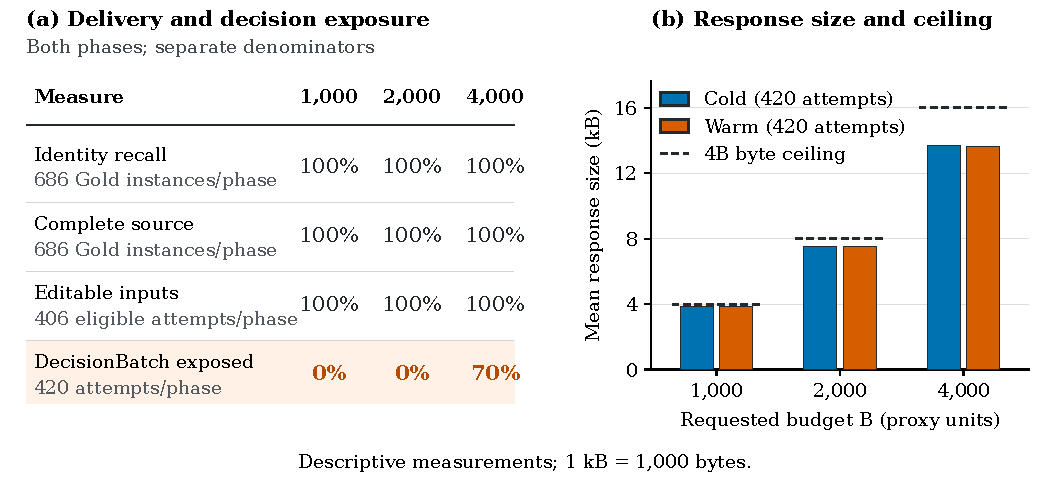
\includegraphics[width=\textwidth]{figures/budget_exposure.pdf}
\caption{预算对不同输出的影响并不相同。左：源码交付、编辑输入成功率和序列化决策记录暴露率采用不同分母（每种条件分别为 686 项源码要求、406 次符合条件的编辑尝试和 420 次总尝试）。冷态与预热态的各项比例一致；两个阶段的数据未合并。右：平均序列化响应字节数均低于计量规则对应的 $4B$ 上限。最低预算已经使源码交付指标达到饱和。}
\label{fig:budget}
\end{figure*}

\subsection{嵌套就绪谓词}
对于 RQ3，按尝试统计的身份、函数体以及函数体加文件元数据谓词，在每种条件下都将 413 次可回答观察判为阳性；完整的编辑输入谓词则判定 406 次为阳性。因此，省略写入资格条件会纳入七次只读观察，占可回答观察的 $7/413=1.69\%$。六种条件下受到影响的 42 次观察，都是同一个只读夹具的重复，不是独立发现的 42 个漏洞。

这一结果规模不大，但具有诊断意义。正确的定位、原始源码和新鲜哈希可能同时存在，编辑却仍不满足准入条件。移除额外的文件元数据 SHA 谓词，在本语料中没有带来进一步区分，因为前一层函数体谓词已经检查了源码窗口哈希。因此，该分析没有识别每个嵌套条件各自独立的因果效应，但确立了一个具体反例：源码可用不等于编辑就绪。

\subsection{预算、可见性与延迟}
在两个缓存阶段中，序列化 \code{DecisionBatch} 的暴露次数在预算 1000 和 2000 下均为 0/420，在预算 4000 下均为 294/420（70\%）。因此，相同的源码召回率并不意味着运行时结构化决策具有相同的可见性。这一发现回答了 RQ4 中关于可见性的部分，但没有将暴露的记录解释为真实任务上的正确决策。

\begin{table*}[t]
\centering\small
\caption{冻结主运行的描述性开销。每行包含 420 次实测调用。延迟分位数按调用汇总；图~\ref{fig:latency} 的经验累积分布函数（ECDF）则使用场景中位数。字节数指序列化 JSON 字节数，不是模型 token 数。}
\label{tab:cost}
\begin{tabular}{@{}rrcrrrr@{}}
\toprule
预算 $B$ & 字节上限 $4B$ & 阶段 & 平均字节数 & p50 (ms) & p95 (ms) & 决策暴露次数\\
\midrule
1000 & 4000 & 冷态 & 3850.14 & 40.186 & 70.913 & 0/420\\
1000 & 4000 & 预热态 & 3849.71 & 27.030 & 51.216 & 0/420\\
2000 & 8000 & 冷态 & 7506.04 & 34.795 & 61.286 & 0/420\\
2000 & 8000 & 预热态 & 7503.97 & 20.738 & 34.736 & 0/420\\
4000 & 16000 & 冷态 & 13667.22 & 25.709 & 56.378 & 294/420\\
4000 & 16000 & 预热态 & 13663.93 & 12.948 & 25.150 & 294/420\\
\bottomrule
\end{tabular}
\end{table*}

\begin{figure}[t]
\centering
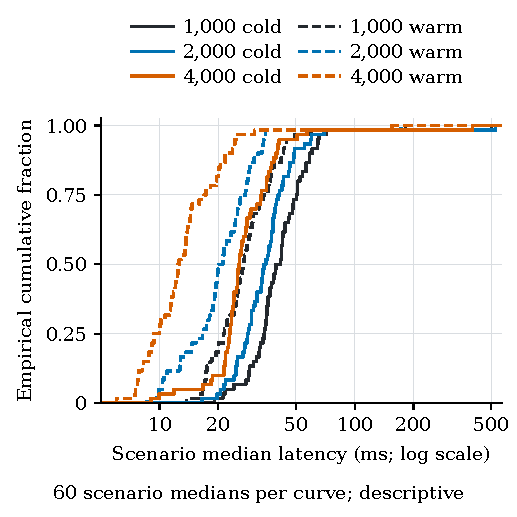
\includegraphics[width=\columnwidth]{figures/latency_ecdf.pdf}
\caption{场景中位数的延迟分布，延迟轴采用对数刻度。六条曲线各包含 60 个中位数，每个中位数来自七次重复调用。颜色表示预算，线型表示执行框架缓存阶段。全部观测中位数均予保留，包括分布的上尾。}
\label{fig:latency}
\end{figure}

在六种条件下，调用延迟中位数介于 12.948 和 40.186\,ms 之间，最大的 p95 为 70.913\,ms。预热态的汇总延迟均低于对应冷态。预算较大的条件在本次运行中也测得更低延迟，但这一关系尚不能证明预算增大带来了加速：固定的预算顺序、打包工作量、共享操作系统缓存和未受控制的主机负载都可能构成混杂因素。能够支持的结论是：在所声明的 debug 构建协议下，该主机上的调用中位数和第 95 百分位数处于数十毫秒量级；单次观察值及部分场景中位数仍延伸至更长的尾部。

综合结果揭示了三种彼此不同的状态：源码要求可以全部得到满足，编辑仍可能不符合准入条件，结构化决策记录也仍可能缺失。将其中任一指标当成通用的就绪分数，都会掩盖返回接口中可观察到的差异。

\section{讨论与效度}
\label{sec:discussion}
\subsection{契约带来的变化}
这一设计的核心结果在于，就绪性不能脱离具体关系来判断。一条记录只能在特定状态和策略下支持特定操作，并不携带一个与上下文无关的“有效”标志。显式保留绑定关系，使系统能够给出三类响应：采纳适用的支持证据、呈现适用的阻断项，或者指出必需的支持证据缺失。后两者都会阻止准入，但对应的后续行动不同。过期源码需要重新观察；当前失败的检查需要解决其失败；缺失的批准则需要履行已配置的批准流程。

这一设计也区分了解释与授权。历史通过记录可以解释某位工作者当时为何采取行动，即使它不能授权验收后续修订。语法边可以指导调查，而不证明语义一致性。已完成的工作项可以描述进展，却不满足验证要求。保留这些记录恰恰有用，因为它们的作用并不等同于验收。

相应的代价是增加状态与响应元数据。修订绑定、生产者键和覆盖字段会占用字节，也需要明确的失效与归约规则。预算实验展示了其中一种表现：完整源码交付可以与决策记录缺失同时出现。分层披露可按需呈现更深层的证据，但它是否改善人或智能体的决策，仍需测量。因此，评价接口是否紧凑，应同时考察精简后哪些要求不再可见，不能只看响应长度。

\subsection{效度威胁}
\paragraph{构念效度。}
Gold 源码交付与编辑输入就绪状态是某些操作的前提，不是补丁正确性的度量。嵌套谓词分析所用的参考定义本身已包含可写性，因此观察到的错误是省略该条件所产生的诊断性结果。同样，序列化决策暴露率衡量的是可供检查的信息。保留的影子评分仍针对同一组开发夹具，不能据此证明独立任务上的决策经过校准。

\paragraph{内部效度。}
固定预算顺序、debug 编译以及未受控制的主机负载，限制了对计时结果的因果解释。新的执行框架不会清空操作系统缓存。运行前后的源码检查与保留的可执行文件有助于确定所报告运行的归属，但不证明执行具有环境封闭性，也不证明每项进程依赖均已被采集。22 项反例重放使用同一保留可执行文件，但每项仅执行一次，且由开发者选定；它们并未对并发调度或潜在失败的空间进行抽样。

\paragraph{外部效度。}
语料是开发过程中编写的合成场景，并按相关的语言家族组织。必需源码异常简短，夹具规模也不能近似独立工业仓库在依赖与构建方面的多样性。重复次数不会增加独立任务数量。本文没有固定模型的问题修复研究、匹配的检索或智能体基线、独立对抗评估或操作者研究。因此，结果支持的是所测试的契约，不能证明在自主性、安全性或可用性方面普遍优于其他系统。

\paragraph{实现边界。}
形式化描述抽象了实现意图；目前没有将每条代码路径与上述公式联系起来的精化证明。文件原子性以单个文件为单位，外部编辑器可能绕过协作式锁定。修订相等所能提供的信息，也仅限于已采集的输入与指纹所覆盖的范围。这些边界明确了契约发挥作用的前提，以及哪些地方需要更强的隔离或测量机制。

\subsection{具有区分力的后续实验}
下游评估应固定模型、任务集合、预算和执行环境，并在独立仓库问题上比较相互匹配的接口。应分别记录补丁正确性、过期编辑拒绝、证据刷新开销、未解决的失败和错误验收。在此基础上，可通过机制干预，在受控故障注入下禁用区分生产者的归约或修订检查，测量假设中的验收错误是否出现。这种设计可以检验因果收益；增加当前夹具的重复运行次数无法回答这一问题。

\section{相关工作}
\label{sec:related}
\paragraph{代码智能体及其接口。}
SWE-bench 使用真实问题与补丁配对以及可执行测试，评估仓库级问题修复 \cite{jimenez2024swebench}。SWE-agent 表明，搜索、读取、编辑和执行接口会影响智能体行为，其中也包括通过反馈拒绝部分无效编辑 \cite{yang2024sweagent}。OpenHands 提供可复用的智能体实现、行动与观察事件、沙箱执行和任务委派 \cite{wang2025openhands}。Agentless 则将定位、修复和验证组织成结构化流水线 \cite{xia2025agentless}。这些系统说明，有必要独立于模型规划策略研究基础设施。\wcode{} 关注操作之间交换的证据是否适用，并通过无模型评估将运行时行为与问题修复性能分开考察。

\paragraph{架构一致性与来源记录。}
软件反射模型（Software Reflexion Models）通过显式映射，将高层结构与从源码导出的模型连接起来，揭示两者的一致与偏离 \cite{murphy1995reflexion}。\wcode{} 将这一已有区别应用于实际运行的工作区，其中声明、语法、语义和运行时观察分别保留各自的含义。W3C PROV-DM 对实体、活动、负有责任的主体以及派生关系建模 \cite{w3c2013provdm}；PROV-AGENT 将来源采集扩展到智能体交互和工作流任务，包括基于 MCP 的采集 \cite{souza2025provagent}。本文关注这些记录何时能够支持当前软件操作。某项记录即使不满足修订、范围或权威性条件，仍可作为具有解释作用的历史记录保留。这是一种领域特定的准入契约，而不是新的来源记录标准。

\paragraph{复用与增量计算。}
Build Systems \`a la Carte 区分调度与重新构建，并通过依赖信息和验证轨迹刻画复用 \cite{mokhov2018buildsystems}。缓存结果必须满足相应输入条件才能使用，这一原则已经成熟。\wcode{} 将同样的推理应用于验证与验收，保留已映射检查、跳过检查、复用结果和新执行之间的差别。其贡献在于这些机制如何在共享的智能体接口运行时中与权威性和生产者范围相互作用，而不是新的增量构建算法。

\paragraph{仓库检索。}
RepoCoder 将仓库检索与迭代生成结合，Repoformer 则学习何时检索可能改善补全 \cite{zhang2023repocoder,wu2024repoformer}。两者都使检索质量与开销成为代码生成的重要因素。本文的交付契约提出一个互补问题：有界响应是否包含标注的身份、原始源码、当前文件元数据和符合条件的编辑输入。这些谓词能够在模型使用响应之前诊断工具层。要比较下游有效性，还需要匹配任务、预算和模型配置。

\paragraph{执行控制与对抗评估。}
CaMeL 将控制流与不可信数据分离，并使用权能（capability）机制对经工具传递的数据流执行策略 \cite{debenedetti2025camel}。AgentDojo 在智能体使用不可信工具输出时，区分合法任务效用与攻击者成功率 \cite{debenedetti2024agentdojo}。\wcode{} 的工作区检查、命令策略和受保护修改，针对的是具体的局部准入边界。选定反例有助于考察这些边界；而针对自适应提示注入的抵抗能力和信息流安全，则需要上述研究所考察的更广泛机制与结果指标。

这些研究方向中的基础机制均已有先行工作。本文研究的系统将它们共享的适用条件显式化，并贯穿源码观察、修改、验证和协调核对。评估在具体接口边界上测量这种组合。

\section{结论}
\label{sec:conclusion}
本文提出 \wcode{}，一个围绕修订绑定证据组织的有状态软件智能体运行时。其准入契约在操作之间保留代码与设计身份、目标覆盖范围、权威性、策略以及生产者冲突。实现通过这些区别，将有界源码交付、乐观修改、验证复用和协调核对连接起来。

保留的可执行文件通过了 22 项选定的契约反例和十一项运行控制检查。其诊断在全部测试预算下交付了每一项标注源码要求和符合条件的编辑输入。同一批数据也说明，交付本身并不足够：只读观察可能满足较弱的就绪谓词；即使源码召回率已经饱和，结构化决策暴露率仍会变化。这些结果确立了限定范围内的实现行为，并为后续研究提供了可审计的基础。下一步实证工作是，在匹配的智能体配置下，检验保持这些契约能否减少错误验收并改善真实仓库任务的结果。

\bibliographystyle{plainnat}
\bibliography{refs}
\appendix
\section{工件身份与复现}
\label{sec:artifact}
主数据集为 \path{frozen-trial/fitness.raw.json}，由归档提交 \code{584abd88}（tree \code{12586d3e}）对应的源码生成。表~\ref{tab:identity} 给出便于定位的短标识；证据清单提供完整哈希、大小和路径。源码归档中的全部 1003 个文件均已与导出版本核对。运行前后清单包含相同的 774 个路径及内容哈希，代码和设计修订均未变化。

\begin{table}[H]
\small\centering
\caption{主工件身份（SHA-256 前缀）。}
\label{tab:identity}
\begin{tabularx}{\columnwidth}{@{}Xl@{}}
\toprule
工件 & SHA-256 前缀\\
\midrule
原始试验报告 & \code{cf2575276eef583d}\\
保留的可执行文件，解压后 & \code{2ffaac58a3fe25ef}\\
可执行文件 gzip 归档 & \code{56b39d3c254318ad}\\
源码 tar 归档 & \code{1ed5157ce1165927}\\
语料定义 & \code{6cf6d8403c48ac25}\\
评价器定义 & \code{43e5455c5758bd11}\\
最终运行核验 & \code{e4c1887409b26ad6}\\
\bottomrule
\end{tabularx}
\end{table}

最初的冻结调用因缺少报告输出目录而以退出码 101 结束，没有产生主原始报告。该进程结束后，所需目录被创建；保留的可执行文件经恢复和哈希核对后直接运行，未重新编译。这次恢复运行以退出码 0 结束，并产生主报告。最初的失败调用仍按失败记录保留。最终核验器的 29 项检查全部通过，并明确处理了两种清单排序约定的差异；原始核验器与恢复执行回执仍可获取。

研究源码包包含汇总、逐场景与谓词分析 CSV、对应的来源哈希清单，以及重新生成矢量图的脚本。随附证据归档保留完整原始报告、源码 tar 归档、压缩可执行文件、核验器，以及各项独立的历史运行。重新分析使用这些保留数据，无需模型服务。单独开展的冻结契约重放为 22 个确切测试各保留一份回执，并核实其使用同一可执行文件且源码未变。历史观察不并入这些结果。

重新执行必须建立新的运行记录。保留的可执行文件面向 macOS arm64，并包含编译时绝对路径；在其他环境重新构建需要兼容的 Rust 工具链与依赖，也会产生新的可执行文件身份。工件文档提供命令与环境细节。公开存档和归档标识应对应实际发布的版本；本地复现包并不隐含这些事项已经完成。

\end{document}
